\chapter{The Tiles IoT Framework}
\label{cha:iot-framework}

In this chapter, the concept of IoT adopted in my research is described. The domain is defined by specifying boundaries, recalling the theories embraced and explaining how this scenario was deployed into the \textit{Tiles IoT framework}. The Tiles framework is composed of a set of tools and a process, guiding the users towards the creation of an IoT application. The concepts described in this chapter are reflected in the research work performed during my PhD, but they also extend into future improvements and developments.


\section{Process}
\label{sec:iot-ideation-process}

The process defined by the Tiles IoT framework is designed to guide non-expert users through the creation of an IoT application. It is divided into five \textit{phases}, reported in Fig.~\ref{fig:ideation-process}. The process starts with the problem elaboration phase and finishes with the production of a low-fidelity prototype of the IoT application.
A brief description of the different phases is provided in the following paragraphs.

\begin{figure}[ptb]
    \centering 
	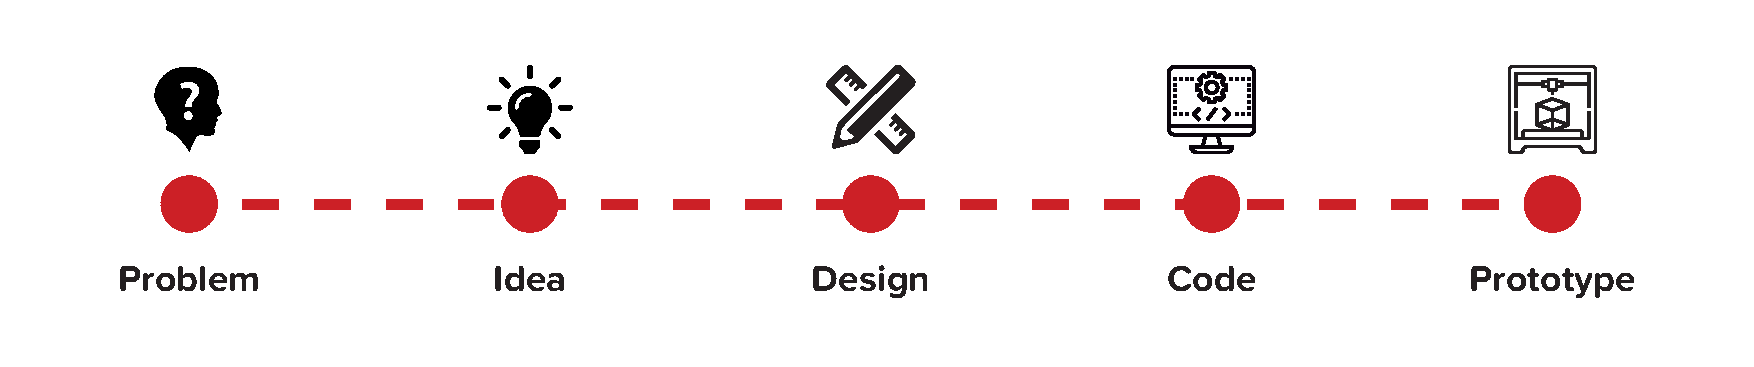
\includegraphics[width=\textwidth]{ideation_process}
	\caption{The process envisioned by the Tiles IoT framework.}
	\label{fig:ideation-process}
\end{figure}

\subsubsection{Problem}
During this first phase, the users select or define a problem that they are willing to address. In order to ease the start of the process, during my work, I often provided the users with a small set of design problems connected to smart cities to choose from.

\subsubsection{Idea}
During this phase, the users combine the different conceptual building blocks that compose a typical IoT application in order to generate smart objects that are relevant to the problem at stake. This brainstorming phase is fuelled by the creativity of the users, who are free to experiment and discuss different solutions and combinations of technology-augmented artefacts. In the papers included in Part II of this thesis and in the remaining of Part I, this phase is referred to as the \textit{brainstorming} or \textit{idea generation} phase.

\subsubsection{Design}
During the \textit{design} phase, the smart objects devised while brainstorming are complemented with a use case scenario. This step guides the users through defining how the objects behave, deciding what the logical connections are among the components of the smart objects and clarifying how the objects interact with each other and with the end-users. The users are also encouraged to reflect on the solution created, analyse it under a different perspective and eventually modify it to match distinct quality criteria.

\subsubsection{Code}
The IoT application design, behaviour and logical connections are translated into code during this phase. I will refer to this phase as the \textit{coding} or \textit{programming} phase throughout the remaining of this thesis.

\subsubsection{Prototype}
The final step consists in physically assembling a low-fidelity prototype of the smart object, which will exhibit the behaviour programmed during the \textit{coding} phase. The prototype created is intended to serve as a physical demonstrator. Efforts are made to improve the speed of development and the possibility of quickly iterating on the implementation, rather than on the complexity of the solution and the long-term stability. I will refer to this phase when discussing \textit{physical prototyping}, \textit{rapid prototyping} or \textit{tangible exploration of ideas} in the next chapters.


\section{Tools}

In order to support the five phases of the Tiles IoT framework process, two toolkits were created from scratch within the Tiles project. When combined, the \textit{Tiles ideation toolkit} and the \textit{RapIoT toolkit} support all the phases of the process defined by the Tiles IoT framework (Fig.~\ref{fig:ideation-process}). The toolkits are composed of an integrated set of technologies and design tools supporting non-experts in a consistent way. The first three phases of \textit{problem elaboration}, \textit{brainstorming} and \textit{design} are supported by the \textit{Tiles ideation toolkit} (see P2, P3 and P4), whereas the last two phases of \textit{programming} and \textit{prototyping} are addressed by the \textit{RapIoT toolkit} (see P6 and P7). A detailed overview of the process in relation to the toolkits is provided in Fig.~\ref{fig:framework}.

\begin{figure}[ptb]
    \centering
	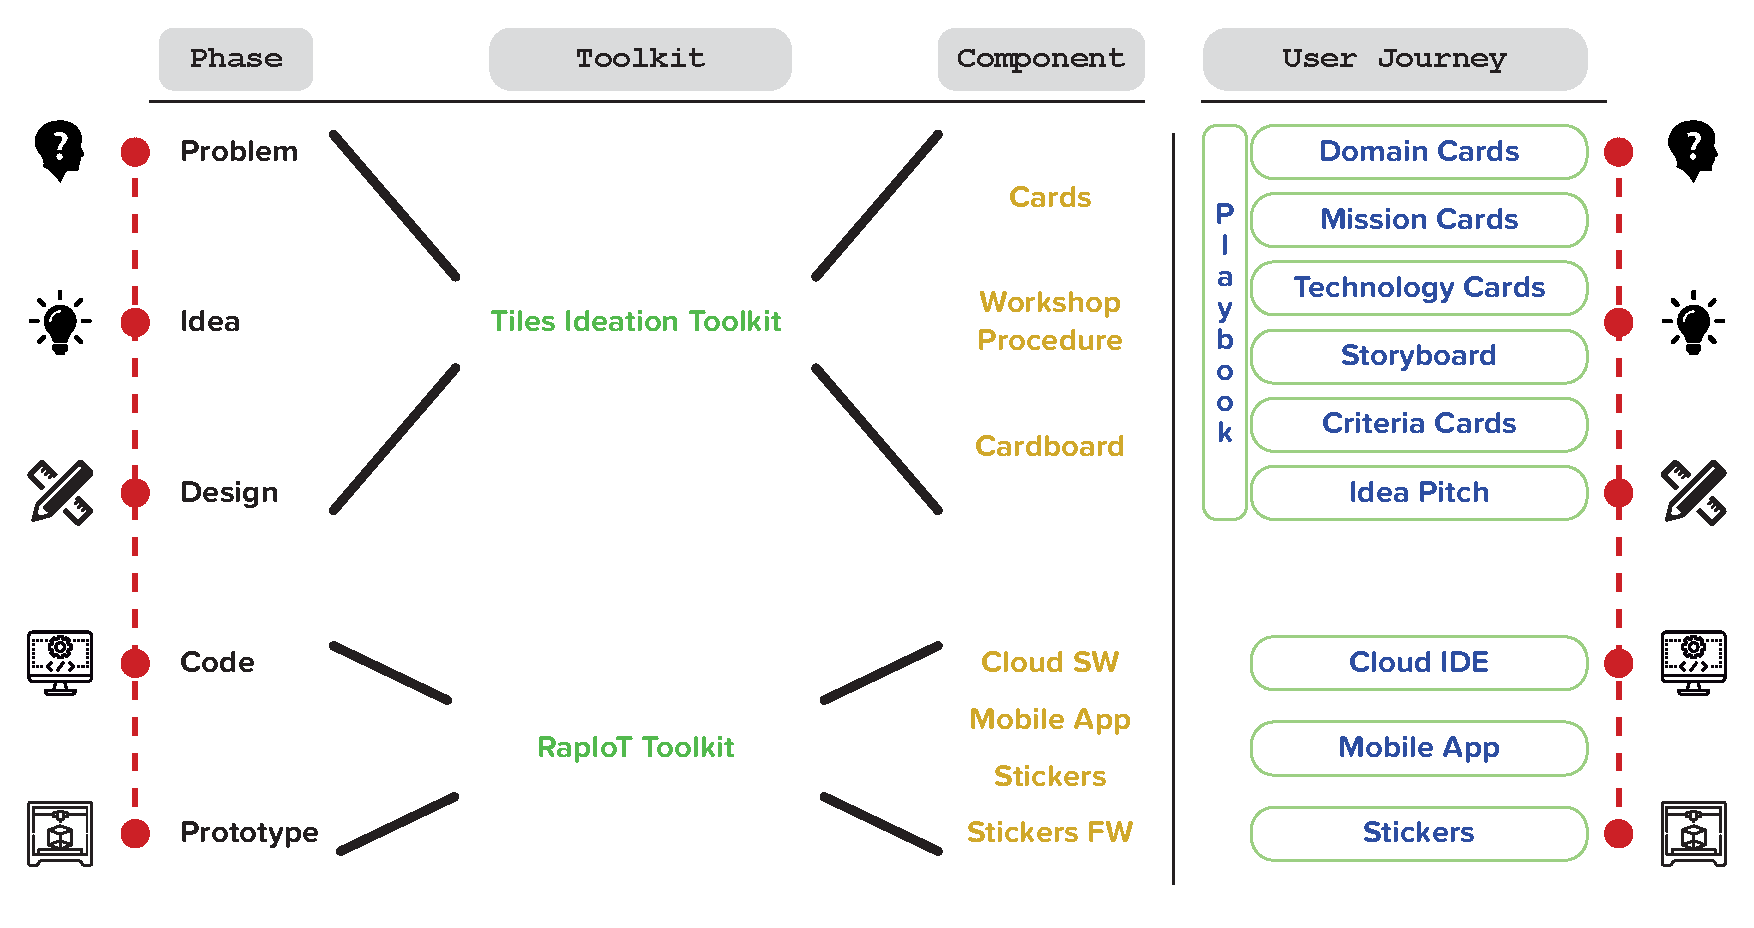
\includegraphics[width=\textwidth]{framework}
	\caption{Mapping of toolkits, components and phases of the Tiles IoT framework.}
	\label{fig:framework}
\end{figure}


The toolkits were designed to support object augmentation as a design strategy for IoT applications. This approach foresees an object as a means of interaction with the \textbf{user} the \textbf{ambient} and the \textbf{network}.

\textbf{User}. When manipulated by the users, augmented objects should be able to sense and distinguish different input commands or gestures (e.g. when a user knocks on, grabs, tilts or shakes an object). As an analogy, similar interaction gestures are widely known and employed in mouse-based interactions (clicking, dragging, double-clicking, etc) and touch interfaces (tapping, double-tapping, swiping, pinching, etc), but they have not been defined for generic object-based interactions.
Augmented objects can also provide sensory feedback and communicate back with the users through actuators, for example, in the form of sound, light or vibration.

\textbf{Ambient}. Objects can sense the ambient where they are positioned and used. Distributed sensing is one of the most popular application domains of IoT. However, in the IoT framework described here, the ability to sense the ambient surrounding the object is not the main function of the object itself. Ambient data like temperature, air pollution and humidity can be used to extend the affordances exposed, enriching the user experience provided by the IoT application.

\textbf{Network}. Connected objects allow integration with services and data streams available on the Internet. Traditionally, IoT applications use networks also to transfer upstream sensor data collected on the field. While these are important use cases that are not discarded by the IoT framework described here, we emphasise the opportunity that a logical \textit{mesh} network topology can offer. A single IoT application can make use of multiple objects that exchange information among themselves. Objects can either sense or provide feedback, or a combination of both. IoT can be more than a network of sensors that only communicates with a central server and presents data through a screen. Ambient sensing, user interaction and feedback are distributed in the environment and interconnected and are part of the same application logic.


\subsection{The Tiles Ideation Toolkit}
\label{sec:tiles-toolkit}

The \textit{Tiles ideation toolkit} (Fig.~\ref{fig:tiles-ideation}) consists of several decks of cards representing the building blocks of an IoT application, a cardboard scaffolding the use of the cards and a workshop technique, which guides the users step by step in the idea generation and design process. The \textit{Tiles ideation toolkit} presents a set of unique characteristics that are not found in already existing card-based toolkits:

\begin{itemize}
    \item \textbf{Velocity}. It allows generating and discussing an idea in less than two hours.
    \item \textbf{Self-containment}. All the materials required are available to the user from the very beginning.
    \item \textbf{Autonomy}. Participants do not need to be supervised or guided by facilitators to complete the creative process.
    \item \textbf{Accessibility}. No technical skills, domain knowledge or design abilities are required.
\end{itemize}

\begin{figure}[ptb]
    \centering 
	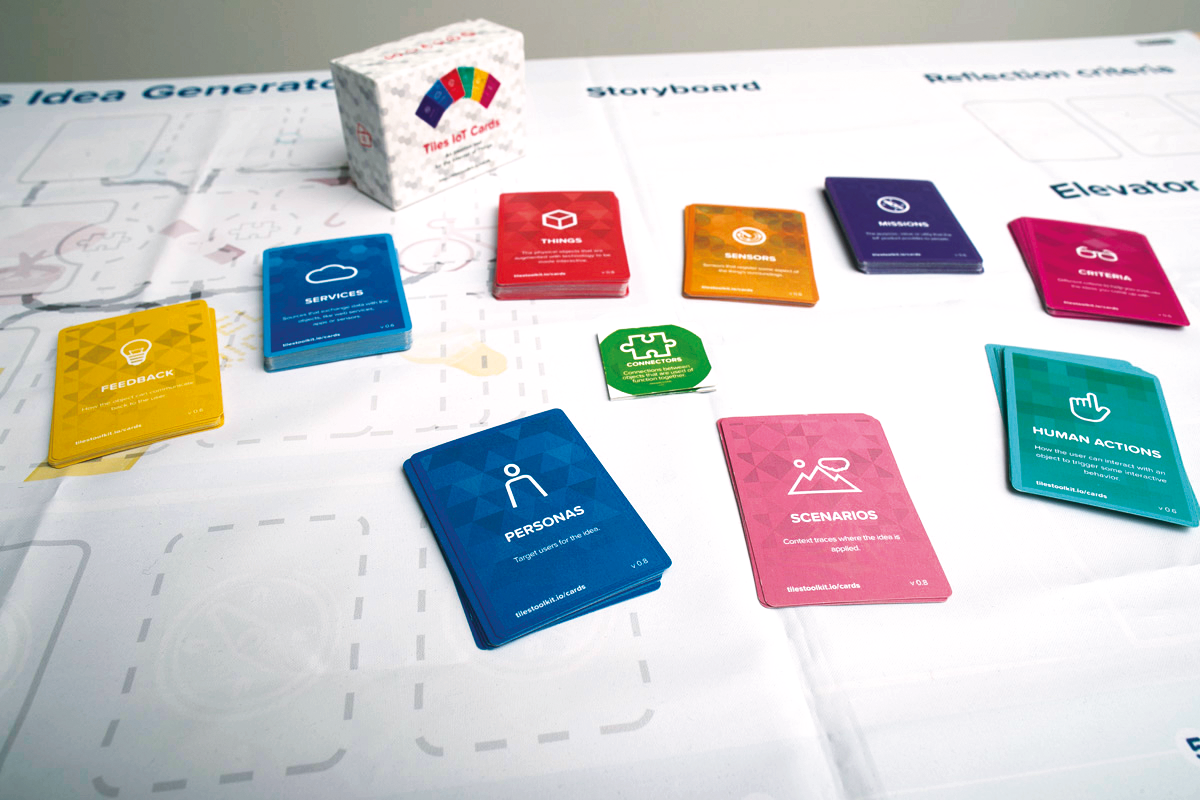
\includegraphics[width=\textwidth]{cards}
	\caption{The last version of the Tiles ideation toolkit. The cardboard and the cards, including the extensions described in P3, are visible in the picture.}
	\label{fig:tiles-ideation}
\end{figure}

In the following I will describe the artefacts and components that constitute the Tiles ideation toolkit. Their relations to the phases of the Tiles IoT framework are also detailed.

\subsubsection{Components}

The phases of \textit{problem elaboration}, \textit{brainstorming} and \textit{design} are addressed by the Tiles ideation toolkit. The workshop technique envisioned by the toolkit is described in detail in the \textit{playbook} visible at the bottom part of the cardboard (Fig.~\ref{fig:cardboard}). The highlighted sectors on the cardboard in Fig.~\ref{fig:cardboard} can be mapped to the first three phases of the Tiles IoT framework process; the cardboard itself and the workshop technique support all the three phases. The individual components of the Tiles ideation toolkit are illustrated in the following.


\begin{figure}[ptb]
    \centering 
	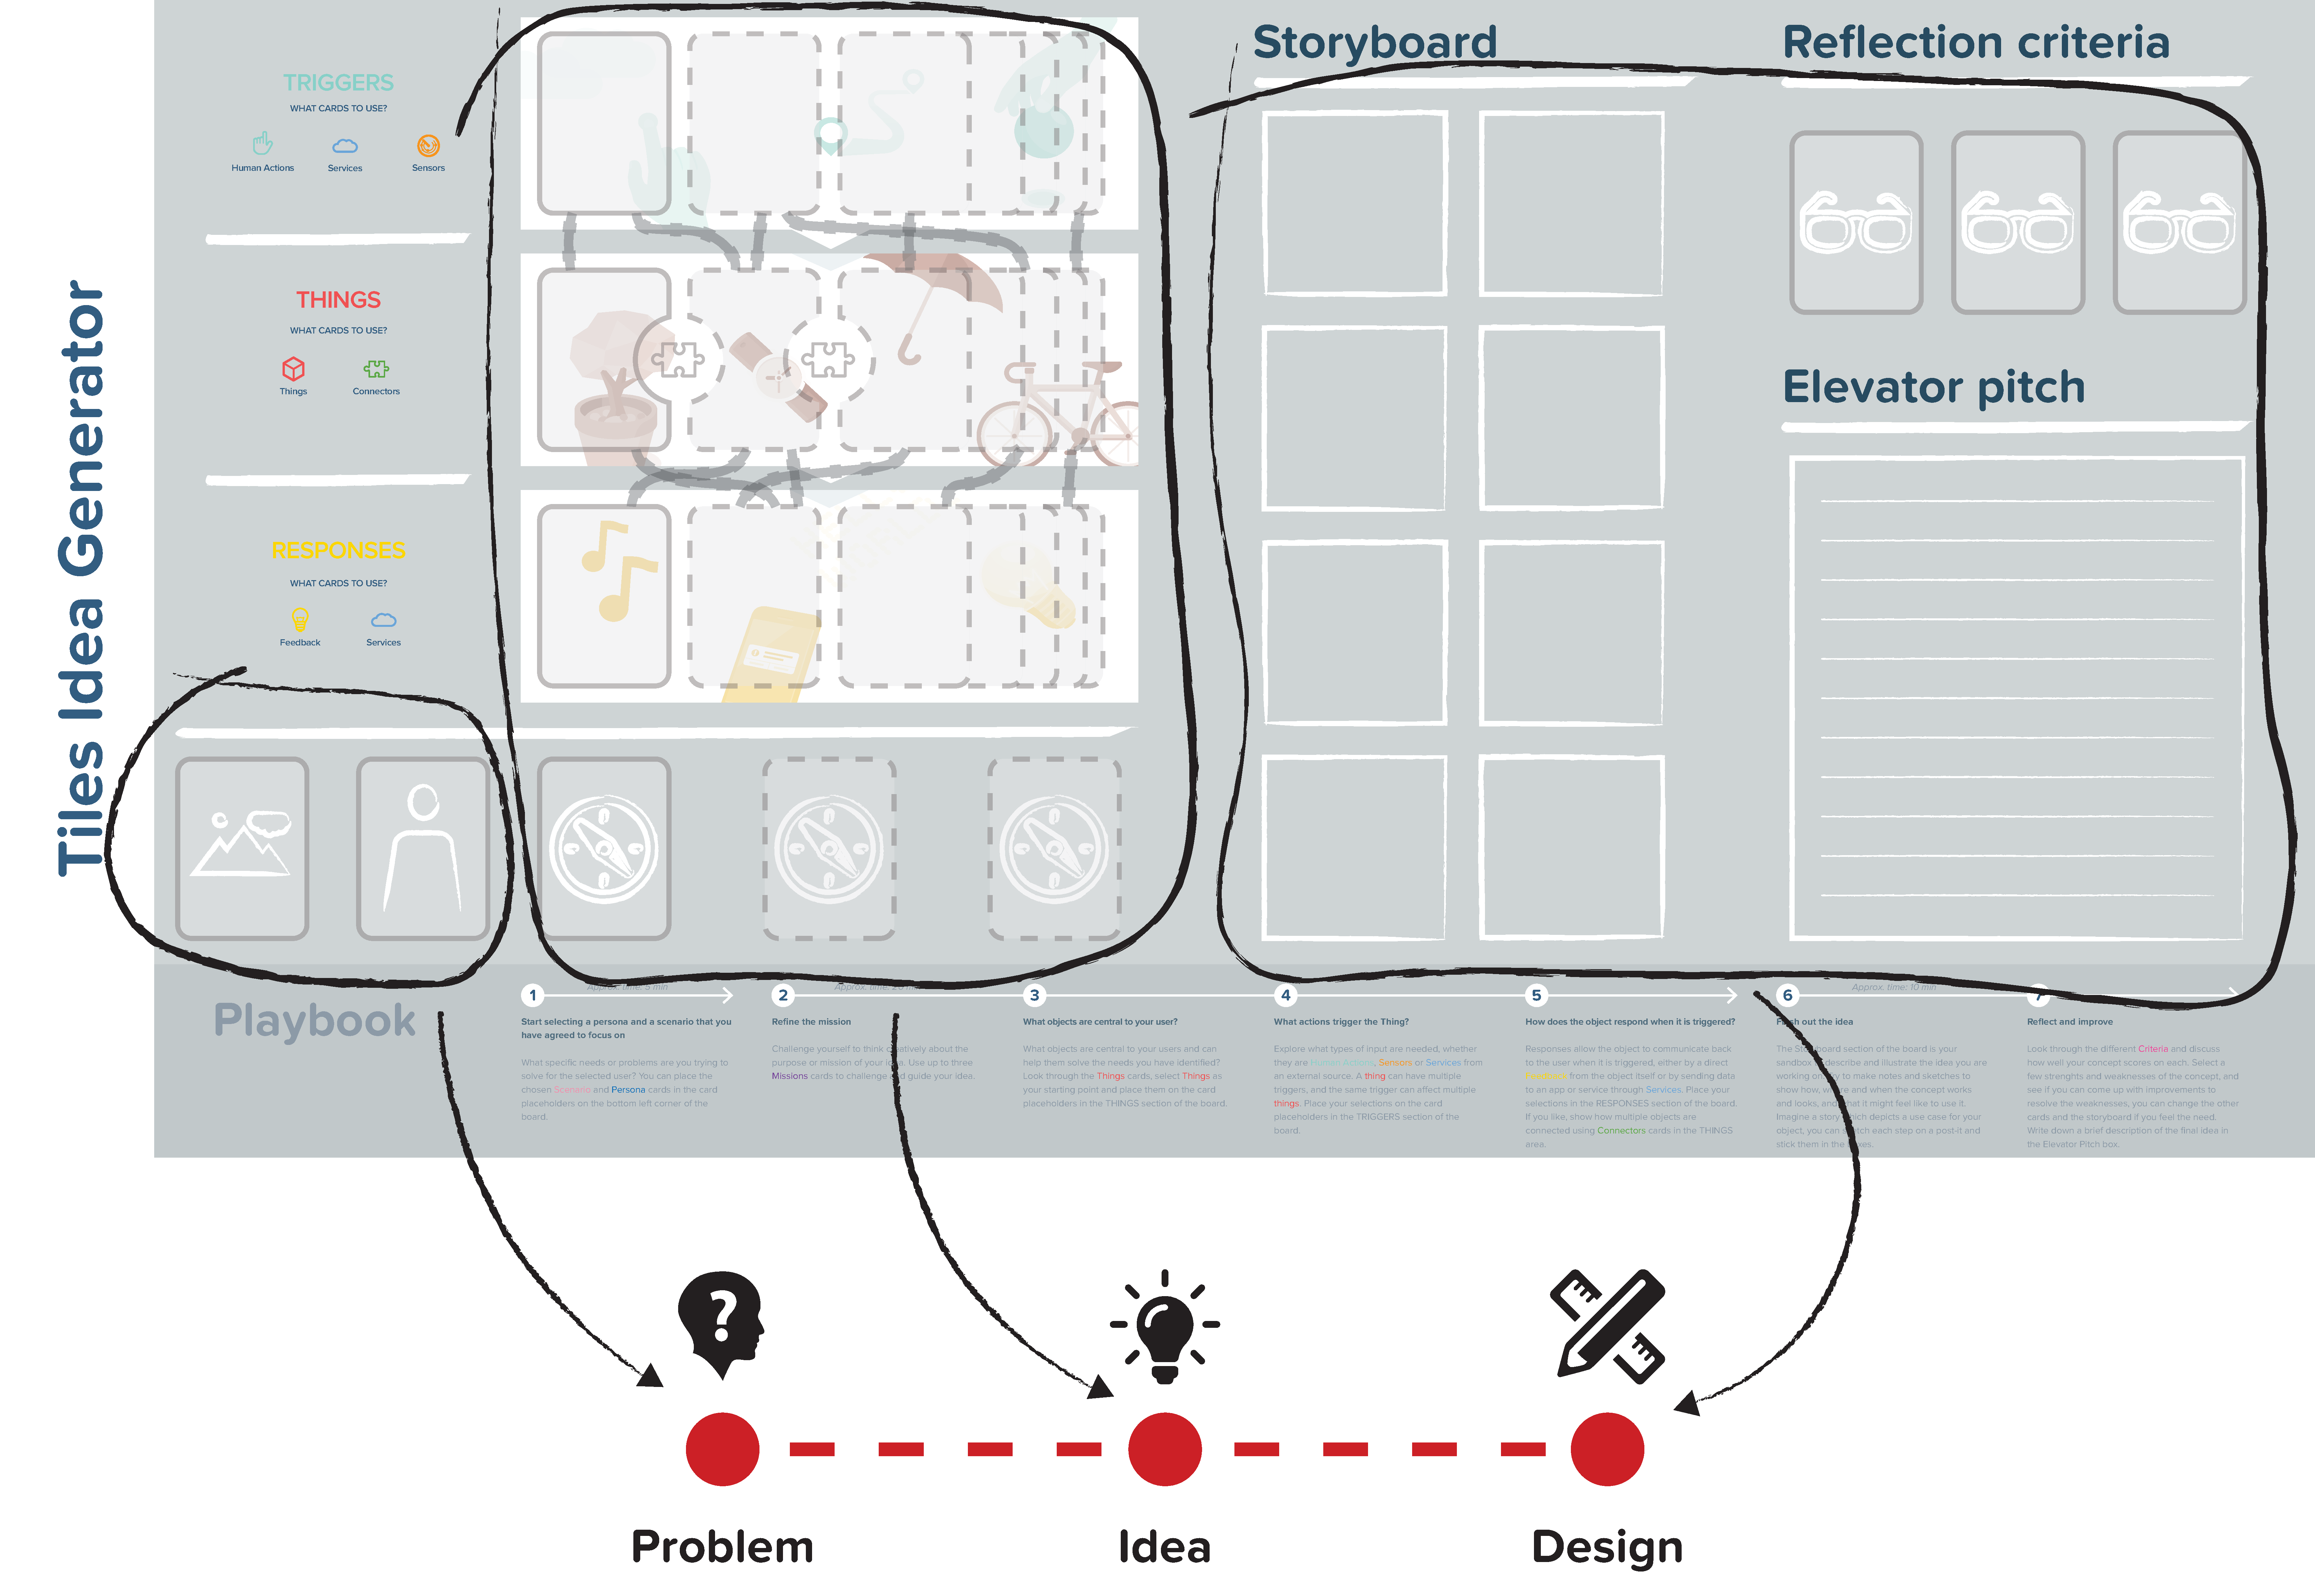
\includegraphics[width=\textwidth]{cardboard}
	\caption{The cardboard included in the Tiles ideation toolkit. The circled sections are connected to the phases of the Tiles IoT framework process.}
	\label{fig:cardboard}
\end{figure}


\textit{\textbf{Personas}} and \textit{\textbf{scenarios}} cards. These cards are used during the initial \textit{problem elaboration} phase, where workshop participants select a target user and a problem to address with their IoT application idea (Fig.~\ref{fig:cards}).

\textit{\textbf{Things}}, \textit{\textbf{sensors}}, \textit{\textbf{services}}, \textit{\textbf{feedback}}, \textit{\textbf{human actions}}, \textit{\textbf{missions}} and \textit{\textbf{connectors}} cards. Workshop participants can define one or more smart objects and model their interactions with the user by combining these decks of cards during the \textit{brainstorming} phase.

\textit{\textbf{Criteria}} cards, \textit{\textbf{storyboard}} and \textit{\textbf{idea pitch}}. In the final \textit{design} phase, workshop participants are encouraged to illustrate a use case for their idea, involving their target user and the augmented objects devised and addressing the problem selected. In order to do that, they sketch a storyboard using post-it notes. The \textit{criteria} cards are also used during this stage to further refine and specialise the idea. Finally, a short text used to pitch the idea is created, thus condensing the ultimate outcome (Fig.~\ref{fig:cardboard}).

For a graphic overview of the final result in terms of creative artefacts and ideas, see the pictures included in P3.

\begin{figure}[ptb]
    \centering 
	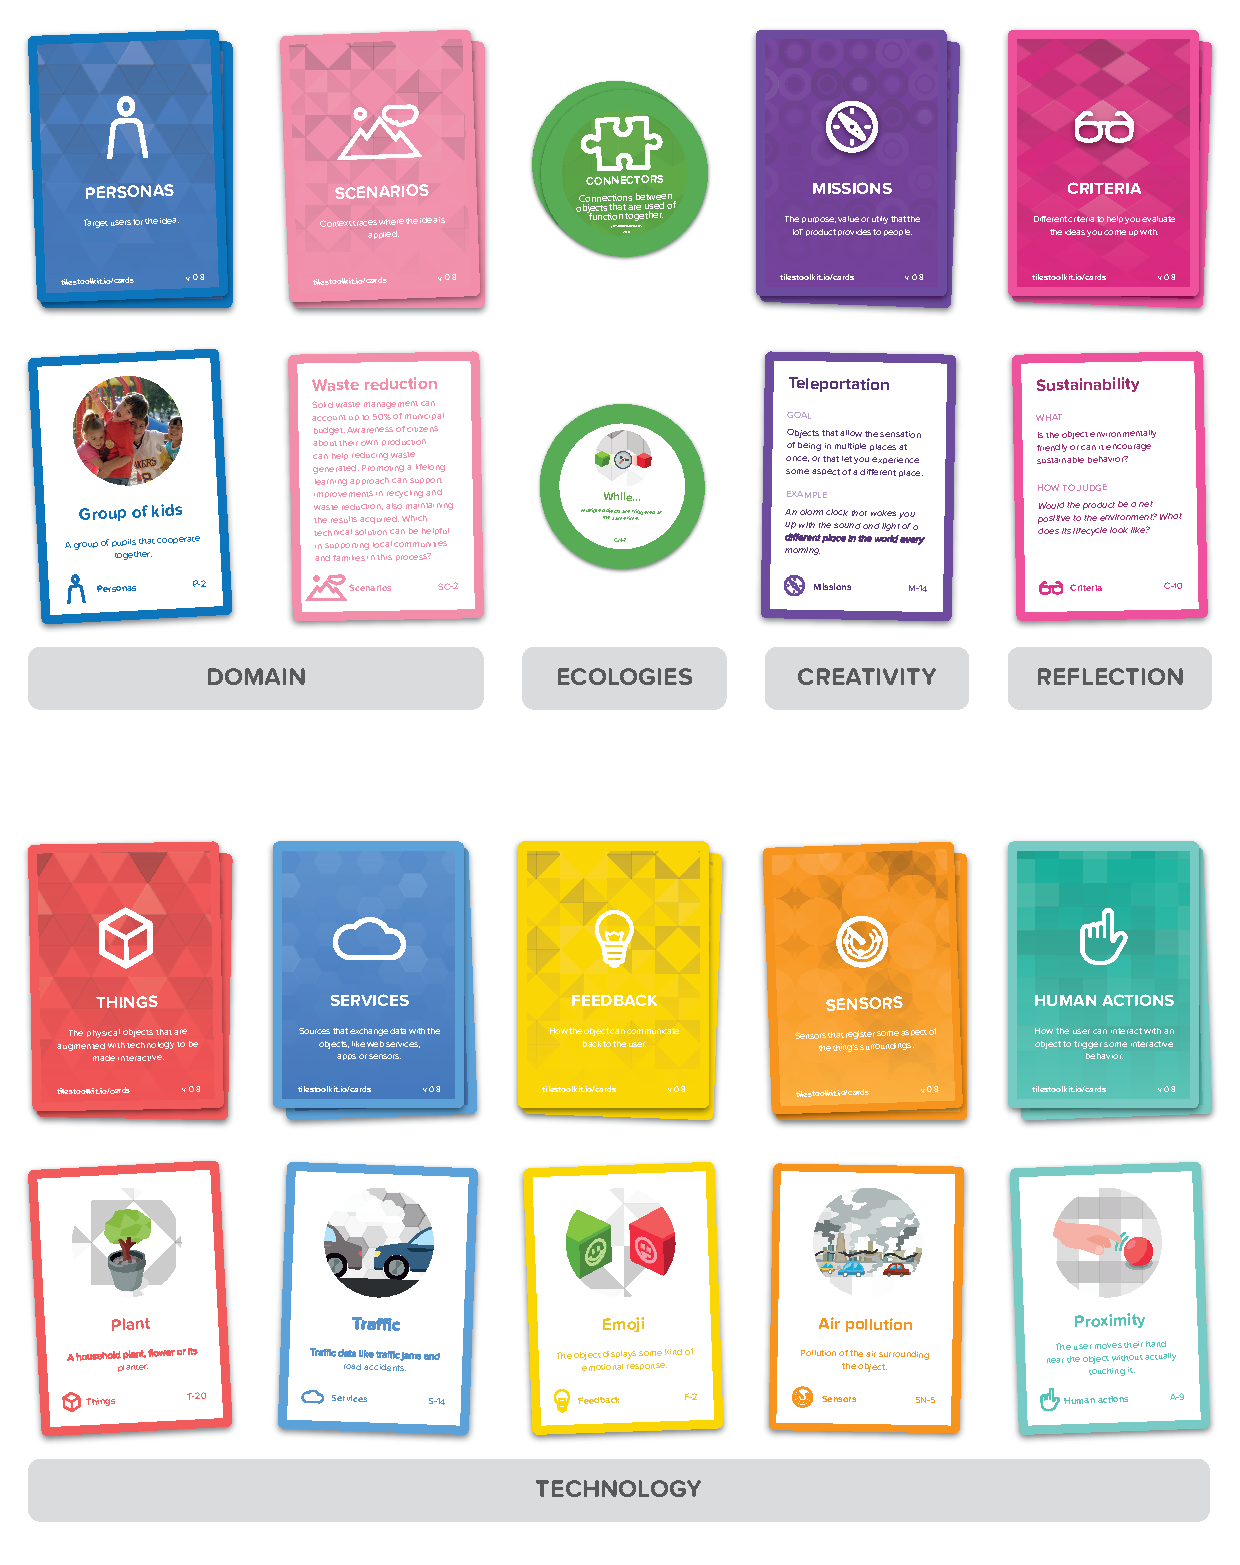
\includegraphics[width=\textwidth]{ideation_cards}
	\caption{Cards included in the Tiles ideation toolkit.}
	\label{fig:cards}
\end{figure}


\subsection{The RapIoT Toolkit}

The \textit{RapIoT toolkit} supports the last two phases of the process defined by the Tiles IoT framework: \textit{coding} and \textit{prototyping} (Fig.~\ref{fig:ideation-process}). These two phases are supported by the use of programmable electronic devices for object augmentation (P7), which function and can be programmed thanks to dedicated software components (P6). Implementing rapid prototyping as object augmentation allows the users to quickly explore the concepts generated during the previous phases. The RapIoT toolkit includes both software and hardware components, allowing the creation of programmable augmented objects.

\subsubsection{Hardware Components}

\textbf{\textit{Stickers}}. As in the other phases, objects remain central and are augmented through electronic \textit{stickers}, which provide sensing and actuation capabilities in a flexible way (Fig.~\ref{fig:stickers}). Modern low-power microcontrollers can be easily embedded in a \textit{sticker} measuring only a few centimetres in length. In a package smaller than 5 x 5 mm, the microcontroller employed includes considerable processing power, communication lines to interact with the attached sensors and actuators and support for secure, IP-based wireless connectivity. These microcontrollers can operate on batteries for years, taking advantage of low-power sleep modes when idle. The \textit{stickers} are battery-powered and connected to the cloud through a gateway, or directly without the need for any other device. Different types of \textit{stickers} can provide different combinations of I/O; many of them can potentially be attached to a single object. They can trigger events while sensing the surrounding ambient or when the users interact with the object that they are attached to. The data packet representing the event is transmitted to the cloud, where the application logic is running. The \textit{stickers} can also consume events received from the cloud (e.g. a command to vibrate). The type and number of events that can be consumed or generated by a \textit{sticker} are only dependent on the type and number of sensors and actuators it has onboard.

\begin{figure}[ptb]
    \centering 
	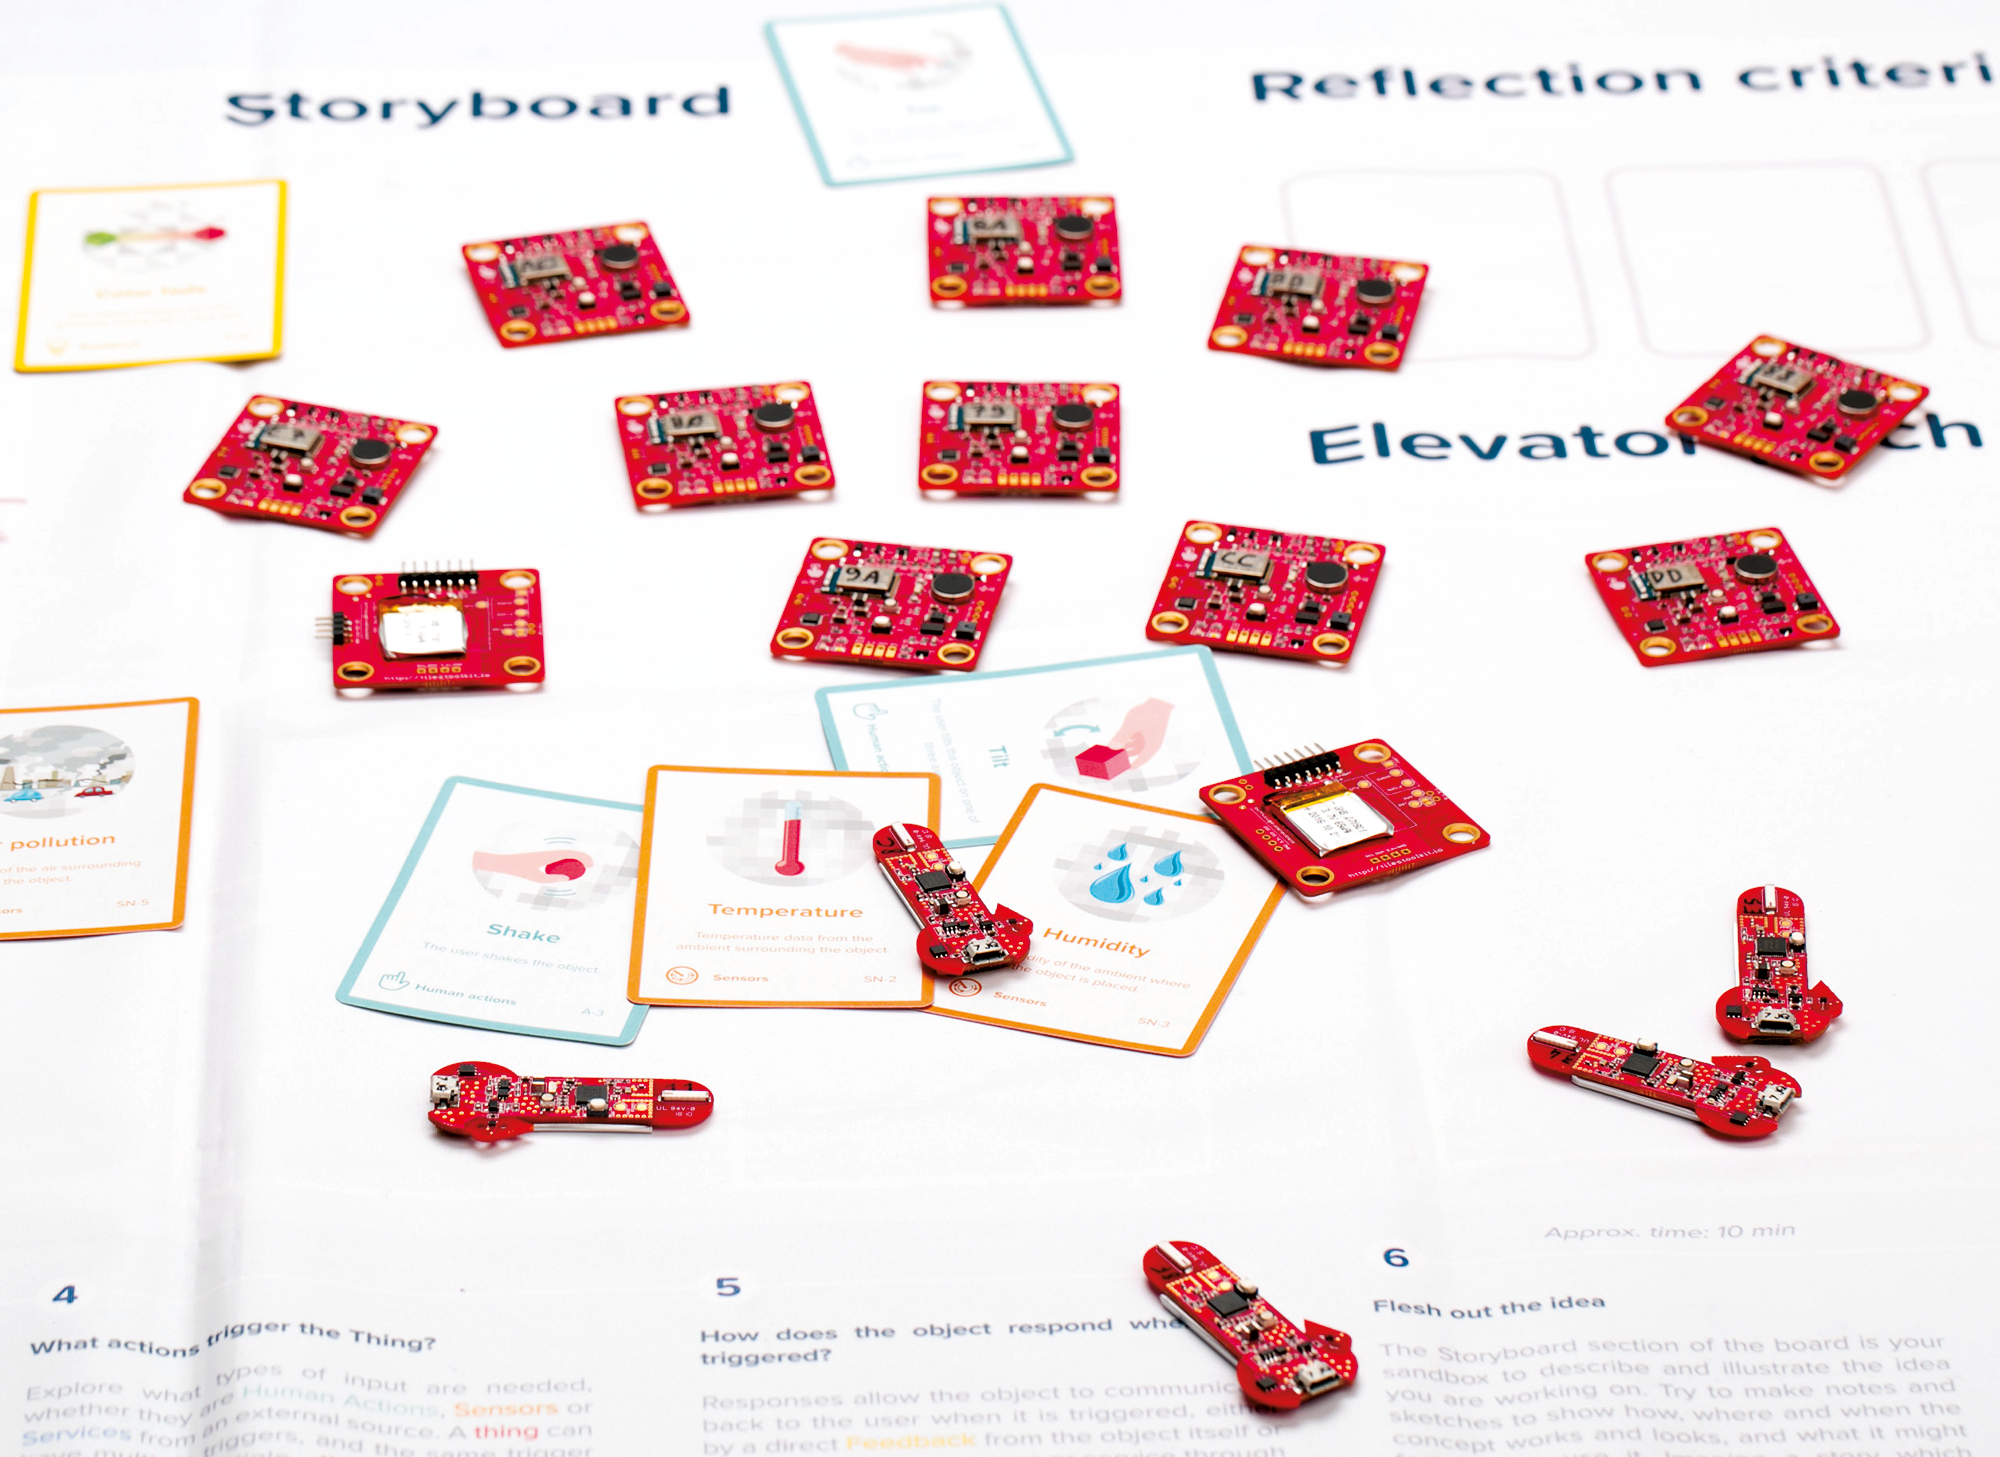
\includegraphics[width=\textwidth]{stickers}
	\caption{Electronic \textit{stickers} employed by the users to prototype the smart objects.}
	\label{fig:stickers}
\end{figure}


\subsubsection{Software Components}

In terms of software, we distinguish two loosely coupled sub-domains: (i) the integrated development environment (IDE) that allows the users to program the application logic and (ii) the platform software stack running on the \textit{stickers}, the cloud and eventually the gateway.

\textbf{\textit{Development Environment}}. The development environment is a cloud-based ambient where the users can program the IoT application logic. The editor used to write the code runs in a browser, sparing the users the installation of any toolchain, driver or software on their personal devices. The programming paradigm employed is a simplified domain-specific language (DSL) based on JavaScript.

\textbf{\textit{Stickers Platform Software Stack}}. The software running on the microcontroller contained in the \textit{stickers} is tasked to fetch data from the sensors attached, command the actuators and expose an API on the network interface. Through the API, the \textit{stickers} can be remotely controlled and can also notify the cloud if new sensor data are available or if any user interaction occurs.

\textbf{\textit{Cloud Platform Software Stack}}. The cloud software acts as a network hub for the \textit{stickers}, exposing their functionalities to the development environment. The development environment, accessible from the browser, is also hosted on the cloud. The cloud IDE is the only interface for the user to program the application logic. To start coding, the user is not required at all to connect any cable or install any software.

\textbf{\textit{Gateway Platform Software Stack}}. The gateway is a device whose main role is to bridge the connectivity between the \textit{stickers} and the cloud. For example, it can provide Bluetooth connectivity to the \textit{stickers} on one side and cellular connectivity on the other, allowing the \textit{stickers} to send and receive events to and from the cloud. We used a smartphone to act as a gateway, and a multi-platform mobile app was developed to handle the connectivity towards the cloud and the \textit{stickers}.

Using IP-based wireless connectivity on the \textit{stickers}, it is possible to reduce the complexity of the gateway, since it would simply need to forward the IP packets between the network interfaces. This way, the gateway would work at a lower level of the ISO/OSI network stack, thus requiring fewer computational resources compared to a routing task involving the full translation of application-level protocols. The use of a gateway can possibly be omitted altogether using new low-power microcontrollers with embedded cellular connectivity. Thanks to these solutions, the \textit{stickers} can have direct access to the cloud like a smartphone.


\section{Integration of the Toolkits in Prototyping}

With the Tiles ideation toolkit and the RapIoT toolkit, we introduced a path of continuity between the phases of \textit{problem definition}, \textit{idea generation} and \textit{design} and the creation of a prototype for quick and tangible exploration of creative ideas.

Connecting these two stages, without limiting the outcome to a simple idea, means supporting the users in the conceptual as well as in the practical stage. This continuum is important for several reasons, as explained by Brown \autocite*{brown_strategy_2005}:

\begin{itemize}
    \item Ideas presented using only words are highly open to interpretation, and require supremely engaging storytelling skills to be relied upon effectively. Words mean different things to different people, especially if they come from different backgrounds.
    \item A prototype, or a demonstrator of the idea, describes a concept in a way that is not open to many interpretations. Physically experiencing the nature of a prototype facilitates convergence towards a shared view.
    \item A prototype is simultaneously an evaluative process (it generates feedback and enables corrections) and a storytelling instrument (it visually describes a strategy or an idea).
\end{itemize}

The goal is not to create a close approximation of the finished product, but to build something that is rough and ready and works, an instrument to elicit feedback, to unlock intuitions from the people \autocite{brown_strategy_2005}.

The Tiles IoT framework guides the users through the different phases in a consistent way. The theoretical concepts, the building blocks of the toolkits and the abstractions employed are introduced gradually and progressively enriched during each phase. This steady learning curve allows capitalising the efforts towards the prototype, avoiding drastic shifts of paradigm or introducing gaps in the knowledge required, which might hinder the creative process.


\section{Lowering the Bar: Non-Experts as Target Users}

The Tiles ideation toolkit and the RapIoT toolkit were designed to keep the entry barriers low, at the same time allowing the users to generate an idea, illustrate it and create a prototype during workshops lasting less than a day.
The target group is represented by \textit{non-expert} users, described in Section~\ref{sec:non-experts}, who have some proficiency in the basic paradigms used by high-level programming languages such as JavaScript abd Python. Upper secondary school students often belong to this category.

The holistic approach of the Tiles IoT framework allows non-experts to actively contribute during tasks that have traditionally required specific technical skills, like low-level programming, assembly and prototyping of electronics for augmented objects.

Since the RapIoT toolkit targets low-complexity applications and non-expert users, it might be beneficial to employ a programming abstraction that requires a lower level of programming skills than the ones usually required by textual programming languages. Visual programming languages like Scratch\footnote{https://scratch.mit.edu/} or Node-RED\footnote{https://nodered.org/} have been successfully employed in rapid prototyping, and their steep learning curve is appreciated by novices \autocite{booth_end-user_2013}. These well-established programming paradigms are easy to use and are understandable interfaces for the configuration of IoT devices \autocite{houben_physikit_2016}.


\section{Identified Values of the Toolkits}

Here, the generic values of the toolkits, identified by Ledo et al. \autocite*{ledo_evaluation_2018} and reported in Chapter~\ref{cha:toolkits}, are recalled and contextualised for the toolkits described in this chapter.

\begin{itemize}
    \item \textbf{G1}: Reducing the Authoring Time and Complexity. The toolkits presented are designed to be used during activities lasting less than a day. Complexity is kept under control by gradually introducing new concepts along the process.
    \item \textbf{G2}: Creating Paths of Least Resistance. The defined rulesets and pathways are present in the toolkits in the form of step-by-step instructions on the playbook and through constraints guiding the coding and prototyping activities.
    \item \textbf{G3}: Empowering New Audiences. The target group of non-expert users, defined as in Section~\ref{sec:non-experts}, are fully involved in the authoring process and represent audiences not traditionally addressed by IoT toolkits.
    \item \textbf{G4}. Integrating with Current Practices. The use of cards and other building blocks that are already familiar to many users facilitates development and integration.
    \item \textbf{G5}. Enabling Replication and Creative Exploration. Ideation, prototyping and replication of creative ideas are used to explore new concepts and tools.
\end{itemize}


\section{Learning from the Past: Tackling Current IoT Challenges}

We are all familiar with what the World Wide Web is and how it works. It is nowadays an essential part of our daily routine, work and leisure. However, we cannot say the same about IoT, despite it being a concept as old as the web. In order to provide the reader with a provocative perspective of the IoT field in its current status, in the following, I will describe the web as if it shares the shortcomings and limitations of the current IoT technologies.

\begin{framed}
Alice just bought a new computer, produced by \textit{BigTechCompany}. She also bought from the same company a cable modem, which will allow her new computer to connect to the telephone line and access the Internet. Using the browser that she found pre-installed on her computer, she quickly discovered that she can only access a limited number of websites, which are associated with or supported by \textit{BigTechCompany}. In order to visit some of the other websites, she needs to install a second browser on her computer, but the website selection will still be quite limited. She wonders how she can connect to the websites associated with \textit{SmallTechCompany}. It seems that a few of the websites of \textit{SmallTechCompany} can be accessed by replacing her cable modem with one produced by \textit{SmallTechCompany}. However, to access all of the websites of \textit{SmallTechCompany}, there is no other way than buying a new computer produced by \textit{SmallTechCompany} itself, which is also the only computer able to run the browser issued by the company.
She decides to buy the required hardware, even if it looks like a waste of money given that she already has a brand-new computer. After a few months, to her great disappointment, \textit{SmallTechCompany} goes out of business, leaving Alice with an expensive computer-shaped paperweight: the websites of \textit{SmallTechCompany} are taken offline, the browser cannot access any other content and the modem does not even connect anymore to the Internet. Alice hopes for someone to take over the work of \textit{SmallTechCompany}, but she gets to know that \textit{SmallTechCompany} did not release any documentation or specification covering the technologies used. That knowledge was condemned to disappear with the company.
\end{framed}

It is difficult to imagine how this fictional scenario could support widespread adoption, growth, accessibility and security. For example, adoption is inhibited by proprietary specifications, accessible only by payment. Growth and accessibility are limited if only a few market players have the resources to develop the technology. Security is affected since it will not be guaranteed if the company licensing the technology goes out of business, leaving the devices of the users exposed \textit{in the wild}.

Many researchers and IoT experts have precisely identified these issues and proposed solutions that build on the aspects that made the web so popular and so different from what described above. This approach was adopted by Guinard and Trifa \autocite*{guinard_building_2016} and was described in their \textit{web of things} architecture. They advocated that the simplicity and openness of the web and its standards are likely what enabled the web we know today. The lingua franca of the web enabled the users to access any webpage without installing anything and has been a major factor in its success. By enabling webpages, browsers, servers and services to all speak the same application language, the integration of a large variety of content was incredibly simplified. Unfortunately, no equivalent enabler has yet been found for devices and applications in IoT \autocite[p. 23]{guinard_building_2016}.

Their pioneering work was not limited to a theoretical exploration. A W3C working group has been established\footnote{https://www.w3.org/WoT/WG/} and is currently active in drafting an open standard based on the \textit{web of things} model. A preliminary implementation of the standard is already in use by the Mozilla IoT gateway\footnote{https://iot.mozilla.org/}, an open-source hub for home automation.

Many other standards, protocols and data models are available in the IoT world. To cite a few examples, the Bluetooth GATT profiles\footnote{https://www.bluetooth.com/specifications/gatt}, the Open Connectivity Foundation oneIoTa\footnote{https://www.oneiota.org/} and the Zigbee Dotdot\footnote{https://www.speakdotdot.com/} all define a mix of APIs, data models and communication protocols to be used with different \textit{things}. Similar ecosystems have been designed and implemented by Apple, Google and Amazon.
These standards are often not as open and accessible as the web ones, and they fall short when addressing IoT under a user-centred perspective. For example, they define APIs to communicate with objects, to allow data sensing and collection, but none of them have yet addressed human interaction primitives and gestures used to manipulate objects, using structured, open and accessible specifications.


\section{Vision for the Tiles IoT Framework}

With the Tiles project, we experimented with and evaluated a user-centred approach to IoT based on physical objects and tangible interfaces. In order to support the target user group of non-experts, our aim was to simplify the setup and deployment tasks of a typical IoT application, providing an intuitive development environment that allows rapid prototyping and fast exploration of ideas. These goals very well fit with the philosophy of the \textit{web of things}, which in addition enables community work, transparency, openness and accessibility. Building future advancements on top of this model will prevent vendor locks and expensive implementations and will allow the Tiles \textit{stickers} to be employed for multiple use cases and by multiple actors, with minimal integration costs even when detached from the RapIoT platform.

Outreach, education and open collaboration are the main principles driving the work of W3C. The adoption of a model backed by an international standards organisation such as the W3C guarantees a solution that is not tied to the fate of a commercial corporation and is royalty-free to use for anybody.